\documentclass[tikz,border=5pt]{standalone}
\usepackage{tikz}
\usepackage[dvipsnames]{xcolor}
\usetikzlibrary{positioning,fit,backgrounds,arrows.meta,calc}

\definecolor{stage1}{RGB}{76,175,80}
\definecolor{stage2}{RGB}{255,152,0}
\definecolor{stage3}{RGB}{100,149,237}
\definecolor{inputred}{RGB}{183,28,28}
\definecolor{outputviolet}{RGB}{103,58,183}
\definecolor{pipelineborder}{RGB}{120,60,60}

\begin{document}
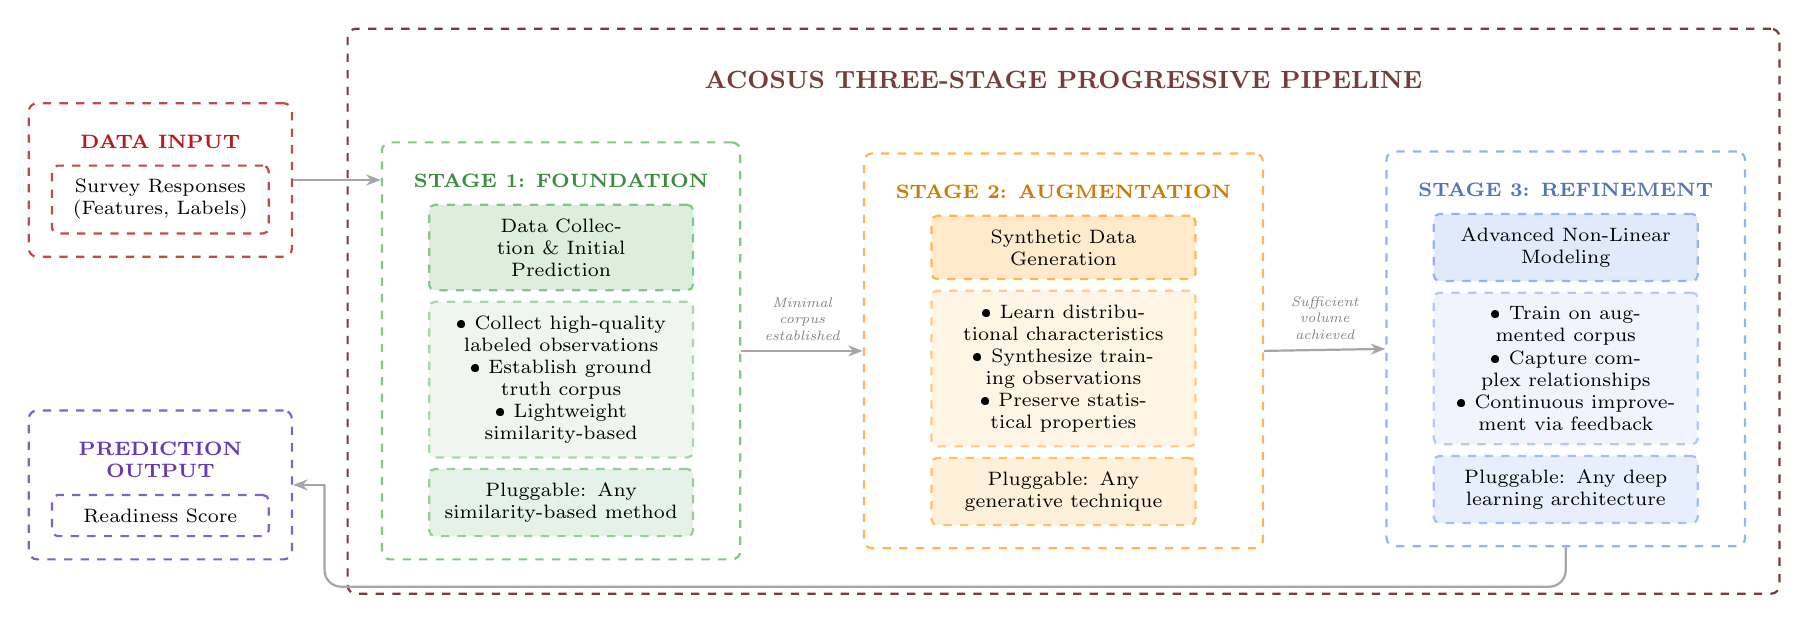
\begin{tikzpicture}[
    node distance=0.3cm,
    inner/.style={rectangle, dashed, thick, rounded corners=2pt, align=center, inner sep=5pt, font=\scriptsize},
    outer/.style={rectangle, dashed, thick, rounded corners=3pt, inner sep=8pt},
    header/.style={inner, fill=#1!20, draw=#1!70},
    content/.style={inner, fill=#1!10, draw=#1!50},
    plug/.style={inner, fill=#1!15, draw=#1!60},
    arrow/.style={-{Stealth[scale=0.8]}, gray!70, thick},
    lbl/.style={font=\tiny\itshape, text=gray, align=center}
]

% Stage 1 inner boxes
\node[header=stage1, text width=3cm] (s1-head) {Data Collection \& Initial\\Prediction};
\node[content=stage1, below=0.12cm of s1-head, text width=3cm] (s1-content) {
    \textbullet\ Collect high-quality labeled observations\\
    \textbullet\ Establish ground truth corpus\\
    \textbullet\ Lightweight similarity-based
};
\node[plug=stage1, below=0.12cm of s1-content, text width=3cm] (s1-plug) {Pluggable: Any\\similarity-based method};
\node[above=0.08cm of s1-head, font=\scriptsize\bfseries, text=stage1!80!black] (s1-title) {STAGE 1: FOUNDATION};
\node[outer, draw=stage1!70, fit=(s1-title)(s1-head)(s1-content)(s1-plug)] (stage1-box) {};

% Stage 2 inner boxes
\node[header=stage2, right=3cm of s1-head, text width=3cm] (s2-head) {Synthetic Data\\Generation};
\node[content=stage2, below=0.12cm of s2-head, text width=3cm] (s2-content) {
    \textbullet\ Learn distributional characteristics\\
    \textbullet\ Synthesize training observations\\
    \textbullet\ Preserve statistical properties
};
\node[plug=stage2, below=0.12cm of s2-content, text width=3cm] (s2-plug) {Pluggable: Any\\generative technique};
\node[above=0.08cm of s2-head, font=\scriptsize\bfseries, text=stage2!80!black] (s2-title) {STAGE 2: AUGMENTATION};
\node[outer, draw=stage2!70, fit=(s2-title)(s2-head)(s2-content)(s2-plug)] (stage2-box) {};

% Stage 3 inner boxes
\node[header=stage3, right=3cm of s2-head, text width=3cm] (s3-head) {Advanced Non-Linear\\Modeling};
\node[content=stage3, below=0.12cm of s3-head, text width=3cm] (s3-content) {
    \textbullet\ Train on augmented corpus\\
    \textbullet\ Capture complex relationships\\
    \textbullet\ Continuous improvement via feedback
};
\node[plug=stage3, below=0.12cm of s3-content, text width=3cm] (s3-plug) {Pluggable: Any deep\\learning architecture};
\node[above=0.08cm of s3-head, font=\scriptsize\bfseries, text=stage3!80!black] (s3-title) {STAGE 3: REFINEMENT};
\node[outer, draw=stage3!70, fit=(s3-title)(s3-head)(s3-content)(s3-plug)] (stage3-box) {};

% Pipeline title (centered above stages)
\path (stage1-box.north west) -- (stage3-box.north east) coordinate[midway] (pipeline-center);
\node[above=0.6cm of pipeline-center, font=\small\bfseries, text=pipelineborder] (pipeline-title) {ACOSUS THREE-STAGE PROGRESSIVE PIPELINE};

% Pipeline outer box
\begin{scope}[on background layer]
\node[outer, draw=pipelineborder, fit=(pipeline-title)(stage1-box)(stage2-box)(stage3-box), inner sep=12pt] (pipeline) {};
\end{scope}

% Input box (aligned to top of pipeline)
\node[inner, fill=white, draw=inputred!80, text width=2.4cm, anchor=north] at ([xshift=-2.8cm]stage1-box.north west |- s1-title.north) (input-inner) {Survey Responses\\(Features, Labels)};
\node[above=0.08cm of input-inner, font=\scriptsize\bfseries, text=inputred] (input-title) {DATA INPUT};
\node[outer, draw=inputred!80, fit=(input-title)(input-inner)] (input-box) {};

% Output box (aligned to bottom of pipeline, same size as input)
\node[inner, fill=white, draw=outputviolet!80, text width=2.4cm, anchor=south] at ([xshift=-2.8cm]stage1-box.south west |- s1-plug.south) (output-inner) {Readiness Score};
\node[above=0.08cm of output-inner, font=\scriptsize\bfseries, text=outputviolet, align=center] (output-title) {PREDICTION\\ OUTPUT};
\node[outer, draw=outputviolet!80, fit=(output-title)(output-inner)] (output-box) {};

% Arrows
\draw[arrow] (input-box.east) -- (stage1-box.west |- input-box.east);
\draw[arrow] (stage1-box.east) -- node[lbl, above] {Minimal\\corpus\\established} (stage2-box.west);
\draw[arrow] (stage2-box.east) -- node[lbl, above] {Sufficient\\volume\\achieved} (stage3-box.west);

% Feedback arrow
\coordinate (turn1) at ([yshift=-0.5cm]stage3-box.south);
\coordinate (turn2) at (turn1 -| output-box.east);
\coordinate (turn3) at ([xshift=0.4cm]output-box.east);
\draw[gray!70, thick, rounded corners=6pt] (stage3-box.south) -- (turn1) -- (turn1 -| turn3) -- (turn3);
\draw[arrow] (turn3) -- (output-box.east);

\end{tikzpicture}
\end{document}